\documentclass[xetex,mathserif,serif]{beamer}
\usepackage{polyglossia}
\setdefaultlanguage[babelshorthands=true]{russian}
\usepackage{minted}
\usepackage{tabu}
\usepackage{moresize}

\useoutertheme{infolines}

\usepackage{fontspec}
\setmainfont{FreeSans}
\newfontfamily{\russianfonttt}{FreeSans}

\definecolor{links}{HTML}{2A1B81}
\hypersetup{colorlinks,linkcolor=,urlcolor=links}

\tabulinesep=0.8mm

\title{Введение в F\#}
\author{Юрий Литвинов}
\date{22.02.2019г}

\begin{document}
	
	\frame{\titlepage}
	
	\section{Введение}
	
	\begin{frame}
		\frametitle{F\#}
		\begin{itemize}
			\item Типизированный функциональный язык для платформы .NET
			\item НЕ чисто функциональный (можно императивный стиль и ООП)
			\item Первый раз представлен публике в 2005 г.
			\item Создавался под влиянием OCaml (практически диалект OCaml под .NET)
			\item Использует .NET CLI
			\item Компилируемый и интерпретируемый
			\item Используется в промышленности, в отличие от многих чисто функциональных языков
		\end{itemize}
	\end{frame}

	\begin{frame}
		\frametitle{Что скачать и поставить}
		\begin{itemize}
			\item Под Windows --- Visual Studio, из коробки
			\item Под Linux
			\begin{itemize}
				\item Rider (студентам бесплатно)
				\item Mono + MonoDevelop + F\# Language Binding, из репозиториев
				\item .NET Core + Visual Studio Code + Ionide
			\end{itemize}
			\item Прямо в браузере: \url{https://dotnetfiddle.net/}
		\end{itemize}
	\end{frame}
	
	\begin{frame}[fragile]
		\frametitle{Пример программы}
		\begin{minted}{fsharp}
printfn "%s" "Hello, world!"
		\end{minted}
		Сравните с
		\begin{minted}{csharp}
namespace HelloWorld
{
    class Program
    {
        static void Main(string[] args)
        {
            System.Console.WriteLine("Hello, world!");
        }
    }
}
		\end{minted}
	\end{frame}

	\section{Let-определения}

	\begin{frame}[fragile]
		\frametitle{let-определение}
		\begin{minted}{fsharp}
let x = 1
let x = 2
printfn "%d" x
		\end{minted}
		можно читать как
		\begin{minted}{fsharp}
let x = 1 in let x = 2 in printfn "%d" x
		\end{minted}
		и понимать как подстановку $\lambda$-терма
	\end{frame}

	\begin{frame}[fragile]
		\frametitle{let-определение, функции}
		\begin{minted}{fsharp}
let powerOfFour x = 
    let xSquared = x * x
    xSquared * xSquared
		\end{minted}
		\begin{itemize}
			\item Позиционный синтаксис
			\begin{itemize}
				\item Отступы строго пробелами
				\item Не надо ";"
			\end{itemize}
			\item Нет особых синтаксических различий между переменной и функцией
			\item Не надо писать типы
			\item Не надо писать \textit{return}
		\end{itemize}
	\end{frame}

	\begin{frame}[fragile]
		\frametitle{Вложенные let-определения}
		\begin{minted}{fsharp}
let powerOfFourPlusTwoTimesSix n =
    let n3 =
        let n1 = n * n
        let n2 = n1 * n1
        n2 + 2
    let n4 = n3 * 6
    n4
		\end{minted}
		\begin{itemize}
			\item \textit{n3} --- не функция!
			\item Компилятор отличает значения и функции по наличию аргументов
			\item Значение вычисляется, когда до \textit{let} <<доходит управление>>, 
					функция --- когда её вызовут. Хотя, конечно, функция --- тоже значение.
		\end{itemize}
	\end{frame}

	\section{Типы}

	\begin{frame}[fragile]
		\frametitle{Типы}
		\begin{minted}{fsharp}
let rec f x =
    if x = 1 then 
        1 
    else 
        x * f (x - 1)
		\end{minted}

		\begin{alertblock}{F\# Interactive}
			\begin{minted}{fsharp}
val f : x:int -> int
			\end{minted}
		\end{alertblock}
		Каждое значение имеет тип, известный во время компиляции
	\end{frame}

	\begin{frame}
		\frametitle{Элементарные типы}
		\begin{itemize}
			\item \textit{int}
			\item \textit{double}
			\item \textit{bool}
			\item \textit{string}
			\item ... (.NET)
			\item \textit{unit} --- тип из одного значения, (). Аналог void.
		\end{itemize}
	\end{frame}
	
	\begin{frame}[fragile]
		\frametitle{Кортежи (tuples)}
		\begin{minted}{fsharp}
let site1 = ("scholar.google.com", 10)
let site2 = ("citeseerx.ist.psu.edu", 5)
let site3 = ("scopus.com", 4)
let sites = (site1, site2, site3)

let url, relevance = site1
let site1, site2, site3 = sites
		\end{minted}
	\end{frame}

	\begin{frame}[fragile]
		\frametitle{Value Tuples}
		\begin{minted}{fsharp}
let origin = struct (0, 0)

let displace struct (x, y) struct (dx, dy)
    = struct (x + dx, y + dy)

displace origin struct (1, 1)
		\end{minted}
	\end{frame}

	\begin{frame}[fragile]
		\frametitle{Лямбды}
		\begin{minted}{fsharp}
let primes = [2; 3; 5; 7]
let primeCubes = List.map (fun n -> n * n * n) primes
		\end{minted}
		\begin{alertblock}{F\# Interactive}
			\begin{minted}{fsharp}
> primeCubes;;
val it : int list = [8; 27; 125; 343]
			\end{minted}
		\end{alertblock}
		\begin{minted}{fsharp}
let f = fun x -> x * x
let n = f 4
		\end{minted}
	\end{frame}


	\begin{frame}
		\frametitle{Списки}
		\begin{small}
			\begin{tabu} {| X[0.9 l p] | X[1 l p] | X[1 l p] |}
				\tabucline-
				Синтаксис                               & Описание                  & Пример                                      \\
				\tabucline-
				\everyrow{\tabucline-}
				$[]$                                    & Пустой список             & $[]$                                        \\
				$[expr; ...; expr]$                     & Список с элементами       & $[1; 2; 3]$                                 \\
				$expr :: list$                          & cons, добавление в голову & $1 :: [2; 3]$                               \\
				$[expr\ ..\ expr]$                      & Промежуток целых чисел    & $[1 .. 10]$                                 \\
				$[for\ x\ in\ list\ \rightarrow\ expr]$ & Генерированный список     & $[for\ x\ in\ 1..99\ \rightarrow\ x\ *\ x]$ \\
				$list\ @\ list$                         & Конкатенация              & $[1; 2]\ @\ [3; 4]$                         \\
			\end{tabu}
		\end{small}
	\end{frame}

	\begin{frame}[fragile]
		\frametitle{Примеры работы со списками}
		\begin{minted}{fsharp}
let oddPrimes = [3; 5; 7; 11]
let morePrimes = [13; 17]
let primes = 2 :: (oddPrimes @ morePrimes)
		\end{minted}
		\begin{minted}{fsharp}
let printFirst primes =
    match primes with
    | h :: t -> printfn "First prime in the list is %d" h
    | [] -> printfn "No primes found in the list"
		\end{minted}
	\end{frame}

	\begin{frame}[fragile]
		\frametitle{Устройство списков}
		\begin{center}
			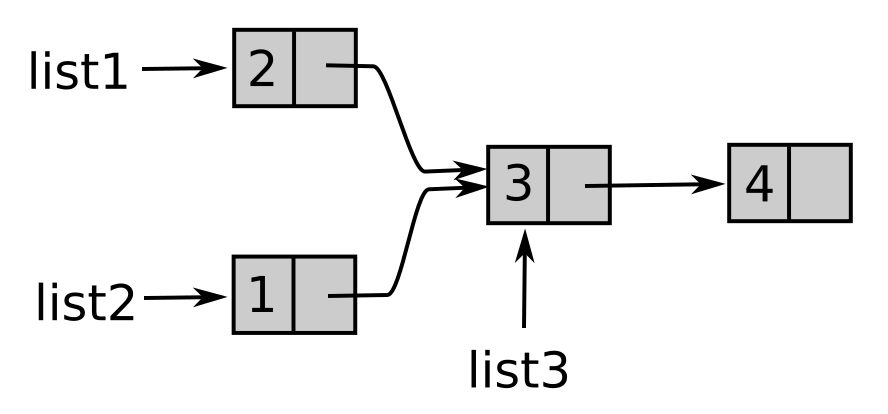
\includegraphics[width=0.4\textwidth]{lists.png}
		\end{center}
		\begin{minted}{fsharp}
let list3 = [3; 4]
let list1 = 2 :: list3
let list2 = 1 :: list3
		\end{minted}
		\begin{itemize}
			\item Списки немутабельны
			\item Cons-ячейки, указывающие друг на друга
			\item cons за константное время, @ --- за линейное
		\end{itemize}
	\end{frame}

	\begin{frame}
		\frametitle{Операции над списками}
		\framesubtitle{Модуль Microsoft.FSharp.Collections.List}
		\begin{small}
			\begin{tabu} {| X[0.5 l p] | X[1 l p] | X[1 l p] | X[0.5 l p] |}
				\tabucline-
				Функция                & Описание                            & Пример                                              & Результат            \\
				\tabucline-
				\everyrow{\tabucline-}
				List.length            & Длина списка                        & $List.length\ [1;2;3]$                              & $3$                  \\
				List.nth               & n-ый элемент списка                 & $List.nth\ [1; 2; 3]\ 1$                            & $2$                  \\
				List.init              & Генерирует список                   & $List.init\ 3 (fun\ i\ \rightarrow\ i * i)$         & $[0; 1; 4]$          \\
				List.head              & Голова списка                       & $List.head\ [1; 2; 3]$                              & $1$                  \\
				List.tail              & Хвост списка                        & $List.tail\ [1; 2; 3]$                              & $[2; 3]$             \\
				List.map               & Применяет функцию ко всем элементам & $List.map\ (fun\ i\ \rightarrow\ i * i)\ [1; 2; 3]$ & $[1; 4; 9]$          \\
				List.filter            & Отбирает нужные элементы            & $List.filter\ (fun\ x\ \rightarrow\ x\ \%\ 2 <> 0)\ [1; 2; 3]$ & $[1; 3]$  \\
				List.fold              & "Свёртка"  & $List.fold\ (fun\ x\ acc\ \rightarrow\ acc * x)\ 1\ [1; 2; 3]$               & $6$                  \\
				List.zip               & Делает из двух списков список пар   & $List.zip\ [1; 2]\ [3; 4]$                          & $[(1, 3); (2, 4)]$   \\
			\end{tabu}
		\end{small}
	\end{frame}
	
	\begin{frame}[fragile]
		\frametitle{Тип Option}
		Либо \textit{Some что-то}, либо \textit{None}, представляет возможное отсутствие значения.
		\begin{minted}{fsharp}
let people = [ ("Adam", None); ("Eve" , None);
    ("Cain", Some("Adam","Eve"));
    ("Abel", Some("Adam","Eve")) ]
		\end{minted}
		\begin{minted}{fsharp}
let showParents (name, parents) =
    match parents with
    | Some(dad, mum) -> 
        printfn "%s, father %s, mother %s" name dad mum
    | None -> printfn "%s has no parents!" name
		\end{minted}
	\end{frame}

	\section{Функции}

	\begin{frame}[fragile]
		\frametitle{Рекурсия}
		\begin{minted}{fsharp}
let rec length l =
    match l with
    | [] -> 0
    | h :: t -> 1 + length t

let rec even n = (n = 0u) || odd(n - 1u)
and odd n = (n <> 0u) && even(n - 1u)
		\end{minted}
	\end{frame}

	\begin{frame}[fragile]
		\frametitle{Каррирование, частичное применение}
		\begin{minted}{fsharp}
let shift (dx, dy) (px, py) = (px + dx, py + dy)
let shiftRight = shift (1, 0)
let shiftUp = shift (0, 1)
let shiftLeft = shift (-1, 0)
let shiftDown = shift (0, -1)
		\end{minted}
		\begin{alertblock}{F\# Interactive}
			\begin{minted}{fsharp}
> shiftDown (1, 1);;
val it : int * int = (1, 0)
			\end{minted}
		\end{alertblock}
	\end{frame}

	\begin{frame}[fragile]
		\frametitle{Зачем --- функции высших порядков}
		\begin{minted}{fsharp}
let lists = [[1; 2]; [1]; [1; 2; 3]; [1; 2]; [1]]
let lengths = List.map List.length lists
		\end{minted}
		или
		\begin{minted}{fsharp}
let lists = [[1; 2]; [1]; [1; 2; 3]; [1; 2]; [1]]
let squares = List.map (List.map (fun x -> x * x)) lists
		\end{minted}
		\vspace{3mm}
		Функции стандартной библиотеки стараются принимать список последним, для каррирования
	\end{frame}

	\begin{frame}[fragile]
		\frametitle{Оператор $|>$}
		\framesubtitle{Pipe forward}
		\begin{minted}{fsharp}
let (|>) x f = f x
		\end{minted}

		\begin{minted}{fsharp}
let sumFirst3 ls = ls |> Seq.take 3 |> Seq.fold (+) 0
		\end{minted}
		вместо
		\begin{minted}{fsharp}
let sumFirst3 ls= Seq.fold (+) 0 (Seq.take 3 ls)
		\end{minted}
	\end{frame}

	\begin{frame}[fragile]
		\frametitle{Оператор $>>$}
		\framesubtitle{Композиция}
		\begin{minted}{fsharp}
let (>>) f g x = g (f x)
		\end{minted}
		\begin{minted}{fsharp}
let sumFirst3 = Seq.take 3 >> Seq.fold (+) 0
let result = sumFirst3 [1; 2; 3; 4; 5]
		\end{minted}
	\end{frame}

	\begin{frame}[fragile]
		\frametitle{Операторы $<|$ и $<<$}
		\framesubtitle{Pipe-backward и обратная композиция}
		\begin{minted}{fsharp}
let (<|) f x = f x
let (<<) f g x = f (g x)
		\end{minted}
		Зачем? Чтобы не ставить скобки:
		\begin{minted}{fsharp}
printfn "Result = %d" <| factorial 5
		\end{minted}
	\end{frame}

	\section{.NET}

	\begin{frame}[fragile]
		\frametitle{Использование библиотек .NET}
		\begin{scriptsize}
			\begin{minted}{fsharp}
open System.Windows.Forms

let form = new Form(Visible = false, TopMost = true, Text = "Welcome to F#")
let textB = new RichTextBox(Dock = DockStyle.Fill, Text = "Some text")
form.Controls.Add(textB)

open System.IO
open System.Net

/// Get the contents of the URL via a web request
let http(url: string) =
    let req = System.Net.WebRequest.Create(url)
    let resp = req.GetResponse()
    let stream = resp.GetResponseStream()
    let reader = new StreamReader(stream)
    let html = reader.ReadToEnd()
    resp.Close()
    html

textB.Text <- http("http://www.google.com")

form.ShowDialog () |> ignore
			\end{minted}
		\end{scriptsize}
	\end{frame}

	\section{Сопоставление шаблонов}
	
	\begin{frame}[fragile]
		\frametitle{Сопоставление шаблонов}
		\begin{minted}{fsharp}
let urlFilter url agent =
    match (url, agent) with
    | "http://www.google.com", 99 -> true
    | "http://www.yandex.ru" , _ -> false
    | _, 86 -> true
    | _ -> false
		\end{minted}

		\begin{minted}{fsharp}
let sign x =
    match x with
    | _ when x < 0 -> -1
    | _ when x > 0 -> 1
    | _ -> 0
		\end{minted}
	\end{frame}

	\begin{frame}[fragile]
		\frametitle{F\# --- не Prolog}
		Не получится писать так:
		\begin{minted}{fsharp}
let isSame pair =
    match pair with
    | (a, a) -> true
    | _ -> false
		\end{minted}
		Нужно так:
		\begin{minted}{fsharp}
let isSame pair =
    match pair with
    | (a, b) when a = b -> true
    | _ -> false
		\end{minted}
	\end{frame}

	\begin{frame}
		\frametitle{Какие шаблоны бывают}
		\begin{small}
			\begin{tabu} {| X[0.9 l p] | X[1 l p] | X[1 l p] |}
				\tabucline-
				Синтаксис                               & Описание                  & Пример                  \\
				\tabucline-
				\everyrow{\tabucline-}
				$(pat, \ldots, pat)$                    & Кортеж                    & $(1, 2, (``3``, x))$    \\
				$[pat; \ldots; pat]$                    & Список                    & $[x; y; 3]$             \\
				$pat :: pat$                            & cons                      & $h :: t$                \\
				$pat\ |\ pat$                           & "Или"                     & $[x]\ |\ [``X``\ ;\ x]$ \\
				$pat\ \&\ pat$                          & "И"                       & $[p] \& [(x, y)]$       \\
				$pat\ as\ id$                           & Именованный шаблон        & $[x]\ as\ inp$          \\
				$id$                                    & Переменная                & $x$                     \\
				$\_$                                    & Wildcard (что угодно)     & $\_$                    \\
				литерал                                 & Константа                 & $239, DayOfWeek.Monday$ \\
				$:?\ type$                              & Проверка на тип           & $:?\ string$            \\
			\end{tabu}
		\end{small}
	\end{frame}

	\section{Юнит-тестирование}

	\begin{frame}
		\frametitle{Юнит-тестирование в F\#}
		\begin{itemize}
			\item Работают все дотнетовские библиотеки (NUnit, MsTest и т.д.)
			\item Есть обёртки, делающие код тестов более ``функциональным'' (FsUnit)
			\item Есть чисто F\#-овские штуки: FsCheck, Unquote 
			\begin{itemize}
				\item на самом деле, не совсем F\#-овские, но в C\# такого нет
			\end{itemize}
		\end{itemize}
	\end{frame}

	\begin{frame}[fragile]
		\frametitle{FsUnit, пример}
		\begin{minted}{fsharp}
module ``Project Euler - Problem 1`` =
    open NUnit.Framework
    open FsUnit

    let GetSumOfMultiplesOf3And5 max =
        seq{3 .. max - 1} 
        |> Seq.fold(fun acc number ->
                    (if (number % 3 = 0 || number % 5 = 0) then
                         acc + number else acc)) 0

    [<Test>]
    let ``Sum of multiples of 3 and 5 to 10 should return 23`` () =
        GetSumOfMultiplesOf3And5(10) |> should equal 23
		\end{minted}
	\end{frame}

	\begin{frame}[fragile]
		\frametitle{FsUnit, матчеры}
		\begin{minted}{fsharp}
1 |> should equal 1
1 |> should not' (equal 2)
10.1 |> should (equalWithin 0.1) 10.11
"ships" |> should startWith "sh"
"ships" |> should not' (endWith "ss")
"ships" |> should haveSubstring "hip"
[1] |> should contain 1
[] |> should not' (contain 1)
anArray |> should haveLength 4

(fun () -> failwith "BOOM!" |> ignore) 
    |> should throw typeof<System.Exception>

shouldFail (fun () -> 5/0 |> ignore)
		\end{minted}
	\end{frame}

	\begin{frame}[fragile]
		\frametitle{FsUnit, ещё матчеры}
		\begin{minted}{fsharp}
true |> should be True
false |> should not' (be True)
"" |> should be EmptyString
null |> should be Null

anObj |> should not' (be sameAs otherObj)

11 |> should be (greaterThan 10)
10.0 |> should be (lessThanOrEqualTo 10.1)

0.0 |> should be ofExactType<float>
1 |> should not' (be ofExactType<obj>)
		\end{minted}
	\end{frame}

	\begin{frame}[fragile]
		\frametitle{FsUnit, и ещё матчеры}
		\begin{minted}{fsharp}
Choice<int, string>.Choice1Of2(42) |> should be (choice 1)

"test" |> should be instanceOfType<string>
"test" |> should not' (be instanceOfType<int>)

2.0 |> should not' (be NaN)

[1; 2; 3] |> should be unique

[1; 2; 3] |> should be ascending
[1; 3; 2] |> should not' (be ascending)
[3; 2; 1] |> should be descending
[3; 1; 2] |> should not' (be descending)
		\end{minted}
	\end{frame}

	\begin{frame}[fragile]
		\frametitle{FsCheck}
		Библиотека, которая берёт функцию и закидывает её случайно сгенерёнными тестами:
		\begin{minted}{fsharp}
open FsCheck

let revRevIsOrig (xs:list<int>) = List.rev(List.rev xs) = xs

Check.Quick revRevIsOrig
// Ok, passed 100 tests.

let revIsOrig (xs:list<int>) = List.rev xs = xs
Check.Quick revIsOrig
// Falsifiable, after 2 tests (2 shrinks) (StdGen (338235241,296278002)):
// Original:
// [3; 0]
// Shrunk:
// [1; 0]
		\end{minted}
	\end{frame}

	\begin{frame}[fragile]
		\frametitle{Unquote}
		Вообще интерпретатор F\#-а, очень полезный для тестирования:
		\begin{minted}{fsharp}
[<Test>]
let ``Unquote demo`` () =
    test <@ ([3; 2; 1; 0] |> List.map ((+) 1)) = [1 + 3..1 + 0] @>

// ([3; 2; 1; 0] |> List.map ((+) 1)) = [1 + 3..1 + 0]
// [4; 3; 2; 1] = [4..1]
// [4; 3; 2; 1] = []
// false
		\end{minted}
	\end{frame}

	\begin{frame}[fragile]
		\frametitle{Foq}
		Ну и, конечно же, mock-объекты:
		\begin{minted}{fsharp}
[<Test>]
let ``Foq demo`` () =
    let mock = Mock<System.Collections.Generic.IList<int>>()
                .Setup(fun x -> <@ x.Contains(any()) @>).Returns(true)
                .Create()

    mock.Contains 1 |> Assert.True
		\end{minted}
	\end{frame}

\end{document}